\chapter{В пространстве наблюдений}

\section{Статический случай} \label{section:filtering:in_observations:static}

Пусть $\xi_* \in L_2^n$ является неизвестной постоянной величиной, от которой линейно зависит математическое ожидание величины $\eta \in L_2^m$:
$$
	\expectation{\eta} = H \xi_* ,
$$
где $H$ --- известная вещественная матрица размера $m \times n$ полного столбцового ранга:
$$
	rank(H) \geq n .
$$
Ковариационная матрица $P_{\eta, \eta}$ вектора $\eta$ является известной положительно определенной матрицей:
$$
	P_{\eta, \eta} = \outerexpectation{\eta}{\eta} > 0 .
$$
Требуется для величины $\xi_*$ построить оценку $\widehat{\xi}$, для которой наименьшего значения достигает отклонение $\Phi_1(\widehat{\xi})$:
\begin{gather*}
	\Phi_1(\widehat{\xi}) = \min_{\xi \sim (\Omega, \Sigma(\eta))} \Phi_1(\xi) , \\
	\Phi_1(\xi) = \Wnorm{\eta - H \xi}{P_{\eta, \eta}^{-1}}^2 = \expectation{\left ( \eta - H \xi \right )^T P_{\eta, \eta}^{-1} \left ( \eta - H \xi \right )} .
\end{gather*}
Поиск минимума отклонения $\Phi_1(\xi)$ выполняется для всех величин $\xi$ измеримых относительно $\left ( \Omega, \Sigma(\eta) \right )$, где
$\Sigma(\eta)$ --- алгебра, порожденная величиной $\eta$.

Определим оценку $\widehat{\xi}$ таким образом, чтобы при каждом фиксированном элементарном исходе $\omega \in \Omega$ величина отклонения
$\Wnorm{\eta(\omega) - H \widehat{\xi}(\omega)}{P_{\eta, \eta}^{-1}}^2$ была минимальной. Легко видеть, что при фиксированном $\omega$ для числовых векторов
$\eta(\omega)$ и $\widehat{\xi}(\omega)$ решение дается методом наименьших квадратов --- вектор $\widehat{\xi}(\omega)$ удовлетворяет нормальной системе:
$$
	H^T P_{\eta, \eta}^{-1} H \widehat{\xi}(\omega) = H^T P_{\eta, \eta}^{-1} \eta(\omega) . 
$$
Поскольку матрица $H$ имеет полный столбцовый ранг, то у матрицы нормальной системы существует обратная матрица, и можно получить выражение для оценки
$\widehat{\xi}(\omega)$ в явном виде:
\begin{equation} \label{equation:filtering:in_observations:static:estimate}
	\widehat{\xi}(\omega) = \left ( H^T P_{\eta, \eta}^{-1} H \right )^{-1} H^T P_{\eta, \eta}^{-1} \eta(\omega) . 
\end{equation}
Легко видеть, что оценка $\widehat{\xi}$ является несмещенной:
\begin{multline*}
	\expectation{\widehat{\xi}}
	= \expectation{\left ( H^T P_{\eta, \eta}^{-1} H \right )^{-1} H^T P_{\eta, \eta}^{-1} \eta}
	= \left ( H^T P_{\eta, \eta}^{-1} H \right )^{-1} H^T P_{\eta, \eta}^{-1} \expectation{\eta} = \\
	%
	= \left ( H^T P_{\eta, \eta}^{-1} H \right )^{-1} H^T P_{\eta, \eta}^{-1} H \xi_*
	= \xi_*
	,
\end{multline*}
поэтому ошибка оценивания $\widehat{\xi} - \xi_*$ совпадает с отклонением оценки $\widehat{\xi}$ от математического ожидания $\expectation{\widehat{\xi}}$
и её можно представить в виде:
\begin{multline*}
	\widehat{\xi} - \xi_*
	= \widehat{\xi} - \expectation{\widehat{\xi}}
	= \left ( H^T P_{\eta, \eta}^{-1} H \right )^{-1} H^T P_{\eta, \eta}^{-1} \eta - \xi_* = \\
	%
	= \left ( H^T P_{\eta, \eta}^{-1} H \right )^{-1} H^T P_{\eta, \eta}^{-1} \eta - \left ( H^T P_{\eta, \eta}^{-1} H \right )^{-1} H^T P_{\eta, \eta}^{-1} H \xi_* \\
	%
	= \left ( H^T P_{\eta, \eta}^{-1} H \right )^{-1} H^T P_{\eta, \eta}^{-1} \left ( \eta - H \xi_* \right )
	= \left ( H^T P_{\eta, \eta}^{-1} H \right )^{-1} H^T P_{\eta, \eta}^{-1} \left ( \eta - \expectation{\eta} \right ) ,
\end{multline*}
откуда ковариационная матрица ошибки оценивания $\widehat{\xi} - \xi_*$ совпадает с ковариационной матрицей оценки $\widehat{\xi}$:
$$
	\expectation{\left ( \widehat{\xi} - \xi_* \right ) \left ( \widehat{\xi} - \xi_* \right )^T}
	= \outerexpectation{\widehat{\xi}}{\widehat{\xi}}
	,
$$
где
\begin{multline} \label{equation:filtering:in_observations:static:estimate_covariance}
	\outerexpectation{\widehat{\xi}}{\widehat{\xi}} = \\
	%
	= \expectation{\left ( H^T P_{\eta, \eta}^{-1} H \right )^{-1} H^T P_{\eta, \eta}^{-1} \left ( \eta - \expectation{\eta} \right ) \left ( \eta - \expectation{\eta} \right )^T  P_{\eta, \eta}^{-1} H \left ( H^T P_{\eta, \eta}^{-1} H \right )^{-1}} = \\
	%
	= \left ( H^T P_{\eta, \eta}^{-1} H \right )^{-1} H^T P_{\eta, \eta}^{-1} \expectation{ \left ( \eta - \expectation{\eta} \right ) \left ( \eta - \expectation{\eta} \right )^T } P_{\eta, \eta}^{-1} H \left ( H^T P_{\eta, \eta}^{-1} H \right )^{-1} = \\
	%
	= \left ( H^T P_{\eta, \eta}^{-1} H \right )^{-1} H^T P_{\eta, \eta}^{-1} P_{\eta, \eta} P_{\eta, \eta}^{-1} H \left ( H^T P_{\eta, \eta}^{-1} H \right )^{-1} = \\
	%
	= \left ( H^T P_{\eta, \eta}^{-1} H \right )^{-1} H^T P_{\eta, \eta}^{-1} H \left ( H^T P_{\eta, \eta}^{-1} H \right )^{-1}
	= \left ( H^T P_{\eta, \eta}^{-1} H \right )^{-1}
	.
\end{multline}

\section{Динамический случай}

\subsection{Последовательность наблюдений}

Пусть $\xi_* \in L_2^n$ по-прежнему является неизвестной постоянной величиной, но наблюдения поступают последовательно в дискретном времени $i = 1, 2, \dots$ в виде
случайных величин $\eta_i \in L_2^p$, математическое ожидание которых неизвестно и линейно зависит от $\xi_*$:
$$
	\expectation{\eta_i} = H_i \xi_* , \\
$$
где $H_i$ --- вещественные матрицы размера $p \times n$, а ковариационные матрицы величин $\eta_i$ являются известными положительно определенными матрицами:
$$
	R_i = \outerexpectation{\eta_i}{\eta_i} > 0 .
$$
Взаимная корреляции между величинами $\eta_i$ отсутствует:
\begin{gather*}
	\outerexpectation{\eta_i}{\eta_j} = 0 , \\
	i \neq j .
\end{gather*}
Необходимо по имеющимся на момент $k$ величинам $\eta_1$, \dots, $\eta_k$ для неизвестной величины $\xi_*$ построить оценку $\widehat{\xi}_k$, для которой
наименьшего значения достигает отклонение $\Phi_2(\xi)$:
\begin{gather*}
	\Phi_2(\widehat{\xi}_k) = \min_{\xi \sim \left ( \Omega, \Sigma(\eta_1, \dots, \eta_k) \right) } \Phi_2(\xi) , \\
	\Phi_2(\xi)
		= \sum_{i=1}^k \Wnorm{\eta_i - H_i \xi}{R_i^{-1}}^2
		= \sum_{i=1}^k \expectation{\left ( \eta_i - H_i \xi \right )^T R_i^{-1} \left ( \eta_i - H_i \xi \right )} .
\end{gather*}
Поиск минимума отклонения $\Phi_2(\xi)$ выполняется для всех величин $\xi$ измеримых относительно $\left ( \Omega, \Sigma(\eta_1, \dots, \eta_k) \right )$, где
$\Sigma(\eta_1, \dots, \eta_k)$ --- алгебра, порожденная величинами $\eta_1$, \dots, $\eta_k$.

\subsection{Блочная форма}

При решении задачи можно воспользоваться результатами раздела \ref{section:filtering:in_observations:static}, если определить случайную величину $\eta_{1|k}$ размера
$m = k \cdot p$, объединяющую величины $\eta_1$, \dots, $\eta_k$:
$$
	\eta_{1|k}
	=
	\begin{pmatrix}
		\eta_1 \\
		\vdots \\
		\eta_k
	\end{pmatrix}
	.
$$
Легко видеть, что математическое ожидание величины $\eta_{1|k}$:
$$
	\expectation{\eta_{1|k}} = H_{1|k} \xi_* ,
$$
где $H_{1|k}$ --- матрица, составленная из матриц $H_i$:
$$
	H_{1|k}
	=
	\begin{pmatrix}
		H_1 \\
		\vdots \\
		H_k
	\end{pmatrix}
	,
$$
и ковариационная матрица величины $\eta_{1|k}$ является блочно диагональной матрицей в виду отсутствия взаимной корреляции между величинами $\eta_i$:
$$
	R_{1|k}
	= \outerexpectation{\eta_{1|k}}{\eta_{1|k}}
	=
	\begin{pmatrix}
		R_1    & 0      & \dots  & 0 \\
		0      & R_2    & \dots  & 0 \\
		\vdots & \vdots & \ddots & \vdots \\
		0      & 0      & \dots  & R_k
	\end{pmatrix}
	,
$$
причем матрица $R_{1|k}$ является положительно определенной, поскольку все диагональные блоки $R_i$ являются положительно определенными.

Легко видеть, что обратная матрица
$$
	R_{1|k}^{-1}
	=
	\begin{pmatrix}
		R_1^{-1} & 0        & \dots  & 0 \\
		0        & R_2^{-1} & \dots  & 0 \\
		\vdots   & \vdots   & \ddots & \vdots \\
		0        & 0        & \dots  & R_k^{-1}
	\end{pmatrix}
	,
$$
поскольку в результате умножения:
$$
	R_{1|k} \cdot R_{1|k}^{-1}
	=
	\begin{pmatrix}
		R_1    & 0      & \dots  & 0 \\
		0      & R_2    & \dots  & 0 \\
		\vdots & \vdots & \ddots & \vdots \\
		0      & 0      & \dots  & R_k
	\end{pmatrix}
	\begin{pmatrix}
		R_1^{-1} & 0        & \dots  & 0 \\
		0        & R_2^{-1} & \dots  & 0 \\
		\vdots   & \vdots   & \ddots & \vdots \\
		0        & 0        & \dots  & R_k^{-1}
	\end{pmatrix}
	=
	\begin{pmatrix}
		I      & 0      & \dots  & 0 \\
		0      & I      & \dots  & 0 \\
		\vdots & \vdots & \ddots & \vdots \\
		0      & 0      & \dots  & I
	\end{pmatrix}
$$
получается единичная матрица.

Определение отклонения $\Phi_2(\xi)$ специально согласовано с отклонением $\Phi_1(\xi)$ таким образом, что:
\begin{multline*}
	\Phi_1(\xi)
	= \Wnorm{\eta_{1|k} - H_{1|k} \xi}{R_{1|k}^{-1}}
	= \expectation{\left ( \eta_{1|k} - H_{1|k} \xi \right )^T R_{1|k}^{-1} \left ( \eta_{1|k} - H_{1|k} \xi \right )} = \\
	%
	= \sum_{i=1}^k \expectation{\left ( \eta_i - H_i \xi \right )^T R_i^{-1} \left ( \eta_i - H_i \xi \right )}
	= \Phi_2(\xi)
	.
\end{multline*}
Таким образом, в соответствии равенством \eqref{equation:filtering:in_observations:static:estimate} искомая оценка $\widehat{\xi}_k$ имеет вид:
\begin{gather}
	\widehat{\xi}_k = \left ( H_{1|k}^T R_{1|k}^{-1} H_{1|k} \right )^{-1} H_{1|k}^T R_{1|k}^{-1} \eta_{1|k} , \notag \\
	\widehat{\xi}_k = P_k H_{1|k}^T R_{1|k}^{-1} \eta_{1|k}
		\label{equation:filtering:in_observations:dynamic:block:current_estimate},
\end{gather}
где в соответствии с равенством \eqref{equation:filtering:in_observations:static:estimate_covariance} матрица $P_k$ является ковариационной матрицей оценки $\widehat{\xi}_k$:
$$
	P_{k} = \outerexpectation{\widehat{\xi}_k}{\widehat{\xi}_k} = \left ( H_{1|k}^T R_{1|k}^{-1} H_{1|k} \right )^{-1} .
$$

\subsection{Итерационная форма}

При поступлении следующего $k+1$-го наблюдения $\eta_{k+1}$ оценка $\widehat{\xi}_{k+1}$ должна иметь вид аналогичный правой части равенства
\eqref{equation:filtering:in_observations:dynamic:block:current_estimate}:
\begin{equation} \label{equation:filtering:in_observations:dynamic:iterative:preliminary_next_estimate}
	\widehat{\xi}_{k+1} = P_{k+1} H_{1|k+1}^T R_{1|k+1}^{-1} \eta_{1|k+1} ,
\end{equation}
где $P_{k+1}$ --- ковариационная матрица оценки $\widehat{\xi}_{k+1}$:
$$
	P_{k+1} = \outerexpectation{\widehat{\xi}_{k+1}}{\widehat{\xi}_{k+1}} = \left ( H_{1|k+1}^T R_{1|k+1}^{-1} H_{1|k+1} \right )^{-1} .
$$
Выражение \eqref{equation:filtering:in_observations:dynamic:iterative:preliminary_next_estimate} для оценки $\widehat{\xi}_{k+1}$ можно преобразовать, используя блочную
форму записи матриц:
\begin{multline} \label{equation:filtering:in_observations:dynamic:iterative:preliminary_estimate}
	\widehat{\xi}_{k+1}
	=
		P_{k+1}
		\begin{pmatrix} H_{1|k}^T & H_{k+1}^T \end{pmatrix}
		\begin{pmatrix}
			R_{1|k} & 0 \\
			0       & R_{k+1}
		\end{pmatrix}^{-1}
		\begin{pmatrix}
			\eta_{1|k} \\
			\eta_{k+1}
		\end{pmatrix} = \\
	%
	=
		P_{k+1}
		\begin{pmatrix} H_{1|k}^T & H_{k+1}^T \end{pmatrix}
		\begin{pmatrix}
			R_{1|k}^{-1} & 0 \\
			0                 & R_{k+1}^{-1}
		\end{pmatrix}
		\begin{pmatrix}
			\eta_{1|k} \\
			\eta_{k+1}
		\end{pmatrix}
	= P_{k+1} \left ( H_{1|k}^T R_{1|k}^{-1} \eta_{1|k} + H_{k+1}^T R_{k+1}^{-1} \eta_{k+1} \right ) = \\
	%
	= P_{k+1} H_{1|k}^T R_{1|k}^{-1} \eta_{1|k} + P_{k+1} H_{k+1}^T R_{k+1}^{-1} \eta_{k+1}
\end{multline}

Полученное выражение для оценки $\widehat{\xi}_{k+1}$ можно преобразовать по схеме, представленной на рисунке
\ref{figure:filtering:in_observations:dynamic:iterative:estimate_transformation}.
\begin{figure}[ht]
	\centering
	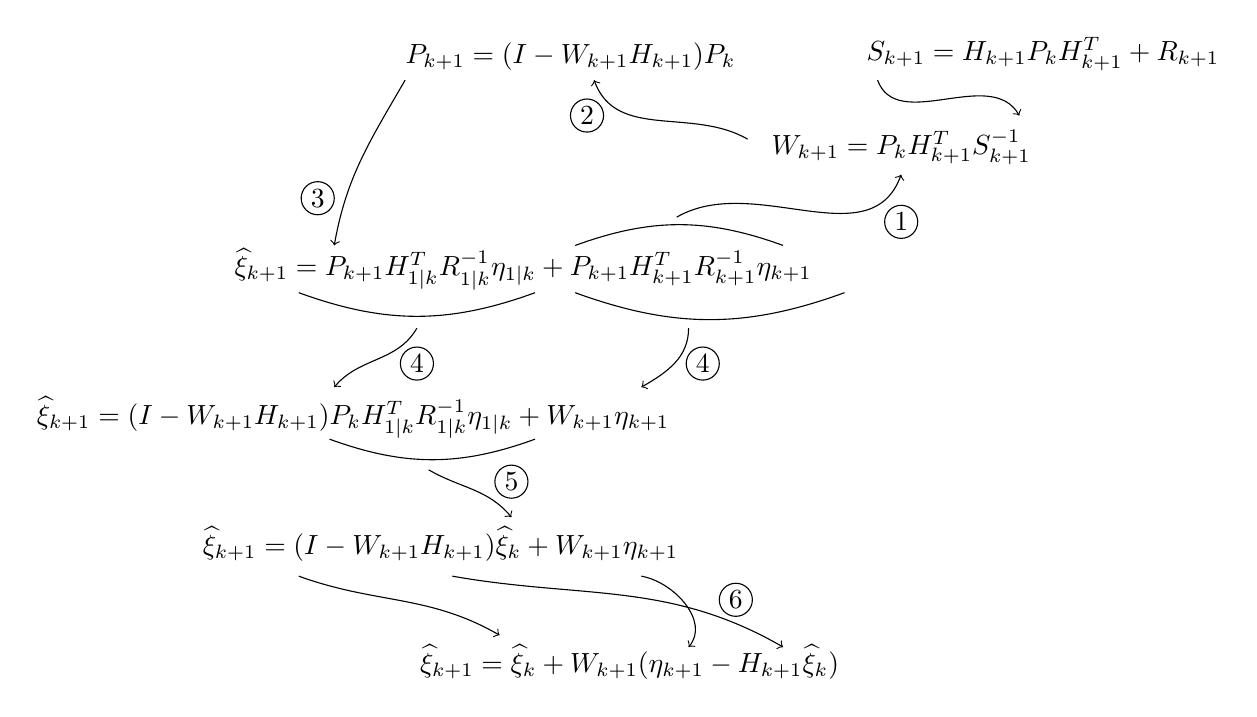
\begin{tikzpicture}[scale=3]
		% исходное выражение
		\node at ( 0, 0 ) {$\widehat{\xi}_{k+1} = P_{k+1} H_{1|k}^T R_{1|k}^{-1} \eta_{1|k} + P_{k+1} H_{k+1}^T R_{k+1}^{-1} \eta_{k+1}$};

		% 1 - W_{k+1}
		\draw ( 0.22, 0.1 ) to [ out = 20, in = 160 ] ( 1.1, 0.1 );
		\draw ( 1.6, 0.2 ) circle [ radius = 0.07 ] node at ( 1.6, 0.2 ) {1};
		\draw [ -> ] ( 0.65, 0.22 ) to [ out = 30, in = -110 ] ( 1.6, 0.4 );
		\node [ above ] at ( 1.6, 0.4 ) {$W_{k+1} = P_k H_{k+1}^T S_{k+1}^{-1}$};

		% S_{k+1}
		\draw [ -> ] ( 1.5, 0.8 ) to [ out = -70, in = 120 ] ( 2.1, 0.65 );
		\node [ above ] at ( 2.2, 0.8 ) {$S_{k+1} = H_{k+1} P_k H_{k+1}^T + R_{k+1}$};	

		% 2 и 3 - P_{k+1}
		\draw ( 0.27, 0.65 ) circle [ radius = 0.07 ] node at ( 0.27, 0.65 ) {2};
		\draw [ -> ] ( 0.95, 0.55 ) to [ out = 150, in = -70 ] ( 0.3, 0.8 );
		\node [ above ] at ( 0.2, 0.8 ) {$P_{k+1} = ( I - W_{k+1} H_{k+1} ) P_k$};
		\draw ( -0.87, 0.3 ) circle [ radius = 0.07 ] node at ( -0.87, 0.3 ) {3};
		\draw [ -> ] ( -0.5, 0.8 ) to [ out = -120, in = 80 ] ( -0.8, 0.1 );

		% 4
		% первое слагаемое
		\draw ( -0.95, -0.1 ) to [ out = -20, in = -160 ] ( 0.05, -0.1 );
		\draw ( -0.45, -0.4 ) circle [ radius = 0.07 ] node at ( -0.45, -0.4 ) {4};
		\draw [ -> ] ( -0.45, -0.25 ) to [ out = -120, in = 50 ] ( -0.8, -0.5 );
		% второе слагаемое
		\draw ( 0.22, -0.1 ) to [ out = -20, in = -160 ] ( 1.36, -0.1 );
		\draw ( 0.76, -0.4 ) circle [ radius = 0.07 ] node at ( 0.76, -0.4 ) {4};
		\draw [ -> ] ( 0.7, -0.25 ) to [ out = -90, in = 30 ] ( 0.5, -0.5 );
		% выражение
		\node [ below ] at ( -0.72, -0.5 ) {$\widehat{\xi}_{k+1} = ( I - W_{k+1} H_{k+1} ) P_k H_{1|k}^T R_{1|k}^{-1} \eta_{1|k} + W_{k+1} \eta_{k+1}$};

		% 5
		\draw ( -0.82, -0.72 ) to [ out = -20, in = -160 ] ( 0.05, -0.72 );
		\draw ( -0.05, -0.9 ) circle [ radius = 0.07 ] node at ( -0.05, -0.9 ) {5};
		\draw [ -> ] ( -0.4, -0.85 ) to [ out = -30, in = 130 ] ( -0.05, -1.05 );
		% выражение
		\node [ below ] at ( -0.35, -1.05 ) {$\widehat{\xi}_{k+1} = (I - W_{k+1} H_{k+1}) \widehat{\xi}_k + W_{k+1} \eta_{k+1}$};

		% 6
		\draw [ -> ] ( -0.95, -1.3 ) to [ out = -20, in = 150 ] ( -0.1, -1.55 );
		\draw ( 0.9, -1.4 ) circle [ radius = 0.07 ] node at ( 0.9, -1.4 ) {6};
		\draw [ -> ] ( -0.3, -1.3 ) to [ out = -10, in = 150 ] ( 1.1, -1.6 );
		\draw [ -> ] ( 0.5, -1.3 ) to [ out = -10, in = 50 ] ( 0.7, -1.6 );
		% выражение
		\node [ below ] at ( 0.45, -1.55 ) {$\widehat{\xi}_{k+1} = \widehat{\xi}_k + W_{k+1} ( \eta_{k+1} - H_{k+1} \widehat{\xi}_k)$};
	\end{tikzpicture}
	\caption{Схема преобразования выражения для оценки $\widehat{\xi}_{k+1}$.}
	\label{figure:filtering:in_observations:dynamic:iterative:estimate_transformation}
\end{figure}

Заметим, что оценка $\widehat{\xi}_{k+1}$ образована двумя слагаемыми: первое слагаемое определяет вклад предыдущих $k$ величин $\eta_1$, \dots, $\eta_k$ в итоговую
оценку $\widehat{\xi}_{k+1}$, а второе слагамое определяет вклад $k+1$-го наблюдения $\eta_{k+1}$. Вес, с которым наблюдение $\eta_{k+1}$ входит в сумму,
определяется коэффициентом усиления $W_{k+1}$:
\begin{equation} \label{equation:filtering:in_observations:dynamic:iterative:preliminary_gain}
	W_{k+1} = P_{k+1} H_{k+1}^T R_{k+1}^{-1} .
\end{equation}

Матрице $W_{k+1}$ можно придать иной вид, если преобразовать первый множитель --- матрицу $P_{k+1}$, используя блочное представление матриц $H_{1|k+1}$ и $R_{1|k+1}$:
\begin{multline} \label{equation:filtering:in_observations:dynamic:iterative:preliminary_next_estimate_covariance}
	P_{k+1} = \left ( H_{1|k+1}^T R_{1|k+1}^{-1} H_{1|k+1} \right )^{-1}
	=
		\left (
			\begin{pmatrix}
				H_{1|k}^T & H_{k+1}^T
			\end{pmatrix}
			\begin{pmatrix}
				R_{1|k} & 0 \\
				0       & R_{k+1}
			\end{pmatrix}^{-1}
			\begin{pmatrix}
				H_{1|k} \\
				H_{k+1}
			\end{pmatrix}
		\right )^{-1} = \\
	%
	=
		\left (
			\begin{pmatrix}
				H_{1|k}^T & H_{k+1}^T
			\end{pmatrix}
			\begin{pmatrix}
				R_{1|k}^{-1} & 0 \\
				0            & R_{k+1}^{-1}
			\end{pmatrix}
			\begin{pmatrix}
				H_{1|k} \\
				H_{k+1}
			\end{pmatrix}
		\right )^{-1}
	= \left ( H_{1|k}^T R_{1|k}^{-1} H_{1|k} + H_{k+1}^T R_{k+1}^{-1} H_{k+1} \right )^{-1} = \\
	%
	= \left ( P_k^{-1} + H_{k+1}^T R_{k+1}^{-1} H_{k+1} \right )^{-1}
	= P_k - P_k H_{k+1}^T \left ( H_{k+1} P_k H_{k+1}^T + R_{k+1} \right )^{-1} H_{k+1} P_k
	,
\end{multline}
где в последнем преобразовании использовалось равенство \eqref{equation:filtering:appendix:inversions:first} леммы об обратной матрице. Подставляя полученное
выражение \eqref{equation:filtering:in_observations:dynamic:iterative:preliminary_next_estimate_covariance} для $P_{k+1}$ в равенство
\eqref{equation:filtering:in_observations:dynamic:iterative:preliminary_gain} для коэффициента усиления $W_{k+1}$, получим:
\begin{multline*}
	W_{k+1}
		= \left ( P_k - P_k H_{k+1}^T \left ( H_{k+1} P_k H_{k+1}^T + R_{k+1} \right )^{-1} H_{k+1} P_k \right ) H_{k+1}^T R_{k+1}^{-1} = \\
	%
	= \left ( P_k H_{k+1}^T - P_k H_{k+1}^T \left ( H_{k+1} P_k H_{k+1}^T + R_{k+1} \right )^{-1} H_{k+1} P_k H_{k+1}^T \right ) R_{k+1}^{-1} = \\
	%
	= P_k H_{k+1}^T \left ( H_{k+1} P_k H_{k+1}^T + R_{k+1} \right )^{-1} \left ( \left ( H_{k+1} P_k H_{k+1}^T + R_{k+1} \right ) -  H_{k+1} P_k H_{k+1}^T \right ) R_{k+1}^{-1} = \\
	%
	= P_k H_{k+1}^T \left ( H_{k+1} P_k H_{k+1}^T + R_{k+1} \right )^{-1} \left ( H_{k+1} P_k H_{k+1}^T -  H_{k+1} P_k H_{k+1}^T + R_{k+1} \right ) R_{k+1}^{-1} = \\
	%
	= P_k H_{k+1}^T \left ( H_{k+1} P_k H_{k+1}^T + R_{k+1} \right )^{-1} R_{k+1} R_{k+1}^{-1}
	= P_k H_{k+1}^T \left ( H_{k+1} P_k H_{k+1}^T + R_{k+1} \right )^{-1} = \\
	%
	= P_k H_{k+1}^T S_{k+1}^{-1}
	,
\end{multline*}
где введено обозначение
\begin{equation} \label{equation:filtering:in_observations:dynamic:iterative:residual_covariance}
	S_{k+1} = H_{k+1} P_k H_{k+1}^T + R_{k+1} .
\end{equation}
С учетом введенного обозначения для матрицы $S_{k+1}$ выражение \eqref{equation:filtering:in_observations:dynamic:iterative:preliminary_next_estimate_covariance} для матрицы
$P_{k+1}$ преобразуется к более компактному виду:
$$
	P_{k+1}
	= P_k - P_k H_{k+1}^T S_{k+1}^{-1} H_{k+1} P_k
	= \left ( I - P_k H_{k+1}^T S_{k+1}^{-1} H_{k+1} \right ) P_k
	= \left ( I - W_{k+1} H_{k+1} \right ) P_k
$$
Таким образом, выражение \eqref{equation:filtering:in_observations:dynamic:iterative:preliminary_estimate} для оценки $\widehat{\xi}_{k+1}$ можно преобразовать к виду:
\begin{gather*}
	\widehat{\xi}_{k+1}
	= \left ( I - W_{k+1} H_{k+1} \right ) P_k H_{1|k}^T R_{1|k}^{-1} \eta_{1|k} + W_{k+1} \eta_{k+1}
	= \left ( I - W_{k+1} H_{k+1} \right ) \widehat{\xi}_k + W_{k+1} \eta_{k+1} , \\
	%
	\widehat{\xi}_{k+1} = \widehat{\xi}_k + W_{k+1} \left ( \eta_{k+1} - H_{k+1} \widehat{\xi}_k \right ) 
	.
\end{gather*}
Из полученного представления следует, что оценка $\widehat{\xi}_{k+1}$ в следующий момент времени $k+1$ складывается из оценки на текущий момент времени
$k$ и поправки, которая с коэффициентом усиления $W_{k+1}$ пропорциональна ошибке экстраполяции наблюдения --- величине $\eta_{k+1} - H_{k+1} \widehat{\xi}_k$,
представляющей разность между следующим наблюдением $\eta_{k+1}$ и его экстраполяцией $H_{k+1} \widehat{\xi}_k$, полученной при обработке предыдущих $k$
наблюдений $\eta_1$, \dots, $\eta_k$.

\subsubsection{Ковариация ошибки экстраполяции наблюдения}

Поскольку величина $\eta_{k+1}$ некоррелирована с величинами $\eta_1$, \dots, $\eta_k$, то она так же не коррелирована с оценкой $\widehat{\xi}_k$, которая является
линейной функцией величин $\eta_1$, \dots, $\eta_k$. Действительно, если оценку $\widehat{\xi}_k$ в соответствии с равенством
\eqref{equation:filtering:in_observations:dynamic:block:current_estimate} представить в виде:
\begin{gather*}
	\widehat{\xi}_k = F_k \eta_{1|k} , \\
	F_k = P_k H_{1|k}^T R_{1|k}^{-1} ,
\end{gather*}
тогда
\begin{multline*}
	\outerexpectation{\eta_{k+1}}{\widehat{\xi}_k}
	= \outerexpectation{\eta_{k+1}}{F_k \eta_{1|k}} = \\
	%
	= \outerexpectation{\eta_{k+1}}{\eta_{1|k}} F_k^T = 0 \cdot F_k^T.
\end{multline*}
Используя полученное равенство вычислим ковариационную матрицу для ошибки экстраполяции $\eta_{k+1} - H_{k+1} \widehat{\xi}_k$:
\begin{multline*}
	\expectation{\left ( \eta_{k+1} - H_{k+1} \widehat{\xi}_k \right ) \left ( \eta_{k+1} - H_{k+1} \widehat{\xi}_k \right )^T} = \\
	%
	= \expectation{\left ( \eta_{k+1} - H_{k+1} \xi_* + H_{k+1} \xi_* - H_{k+1} \widehat{\xi}_k \right ) \left ( \eta_{k+1} - H_{k+1} \xi_* + H_{k+1} \xi_* - H_{k+1} \widehat{\xi}_k \right )^T} = \\
	%
	= \expectation{\left ( \eta_{k+1} - H_{k+1} \xi_* - H_{k+1} ( \widehat{\xi}_k - \xi_* ) \right ) \left ( \eta_{k+1} - H_{k+1} \xi - H_{k+1} ( \widehat{\xi}_k - \xi_* ) \right )^T} = \\
	%
	= \expectation{\left ( \eta_{k+1} - \expectation{\eta_{k+1}} - H_{k+1} \left ( \widehat{\xi}_k - \expectation{\widehat{\xi}_k} \right ) \right ) \left ( \eta_{k+1} - \expectation{\eta_{k+1}} - H_{k+1} \left ( \widehat{\xi}_k - \expectation{\widehat{\xi}_k} \right ) \right )^T} = \\
	%
	\shoveleft{
		= \expectation{\left ( \eta_{k+1} - \expectation{\eta_{k+1}} \right ) \left ( \eta_{k+1} - \expectation{\eta_{k+1}} \right )^T} -
	} \\
	- \expectation{\left ( \eta_{k+1} - \expectation{\eta_{k+1}} \right ) \left ( \widehat{\xi}_k - \expectation{\widehat{\xi}_k} \right )^T H_{k+1}^T} - \\
	- \expectation{H_{k+1} \left ( \widehat{\xi}_k - \expectation{\widehat{\xi}_k} \right ) \left ( \eta_{k+1} - \expectation{\eta_{k+1}} \right )^T} + \\
	\shoveright{
		+ \expectation{H_{k+1} \left ( \widehat{\xi}_k - \expectation{\widehat{\xi}_k} \right ) \left ( \widehat{\xi}_k - \expectation{\widehat{\xi}_k} \right )^T H_{k+1}^T}
		=
	} \\
	%
	= R_{k+1} + H_{k+1} \outerexpectation{\widehat{\xi}_k}{\widehat{\xi}_k} H_{k+1}^T = \\
	= R_{k+1} + H_{k+1} P_k H_{k+1}^T .
\end{multline*}
Заметим, что полученное выражение совпадает с правой частью равенства \eqref{equation:filtering:in_observations:dynamic:iterative:residual_covariance}, откуда следует, что
матрица $S_{k+1}$:
$$
	S_{k+1}
	= R_{k+1} + H_{k+1} P_k H_{k+1}^T
	= \expectation{\left ( \eta_{k+1} - H_{k+1} \widehat{\xi}_k \right ) \left ( \eta_{k+1} - H_{k+1} \widehat{\xi}_k \right )^T}
	.
$$
является ковариационной матрицей для ошибки экстраполяции $\eta_{k+1} - H_{k+1} \widehat{\xi}_k$.
